The system consists of a thrust vectoring rocket with Inertial measurment Unit (IMU) GY - 87. It was readily available from the university's supplies.
Multiple physical and software constraints have to be taken into account when implementing the system. For the software part, the controller implementation was the same as the inverted pendulum with the variables values changed to fit the rocket controller.

\section{Sensors}
The response time of the sensors are an important feature when ensuring the stability of the rocket. It cannot be too slow, otherwise the system will react to late to any angle variation. The servomotors system dynamics are described in \autoref{ssc:Servomotors}.

As it can be seen in the Arduino code "rocket controller code" included with this report, the gyroscope/angle sensor needs to write 14 bytes into the Arduino register. The code to use the MPU 6050 was done by Brainergizer \cite{web:gyro_angle}. Since the gyroscope has an internal clock of 1MHz \cite{datasheet:MPU-6050}, the sampling time for the angle sensor is $\frac{14 \cdot 8}{1 \cdot 10^{6}} = 1.12 \cdot 10^{-4}$ seconds or a sampling rate of approximatively 8.9 KHz. The processing time of the 16MHz micro-controller is considered insignificant, since there is no time-intensive sensor processing tasks in the code.

\section{PCBs}
To control the rocket and to fire it safely, 3 different PCB (Printed Circuit Boards) were designed. A logic board, a Power Supply Unit (PSU) and an electric igniter. The logic board and the PSU are stacked on top of each other and the battery is inserted between the two cards to optimize space. All cards schematics are available in the included "PCB schematics folder".

\subsection{Logic board}
The logic board hosts the Arduino Nano micro-controller, the battery connector, the servo output, the IMU and four indicator LEDs.

\begin{figure} [h]
	\centering
	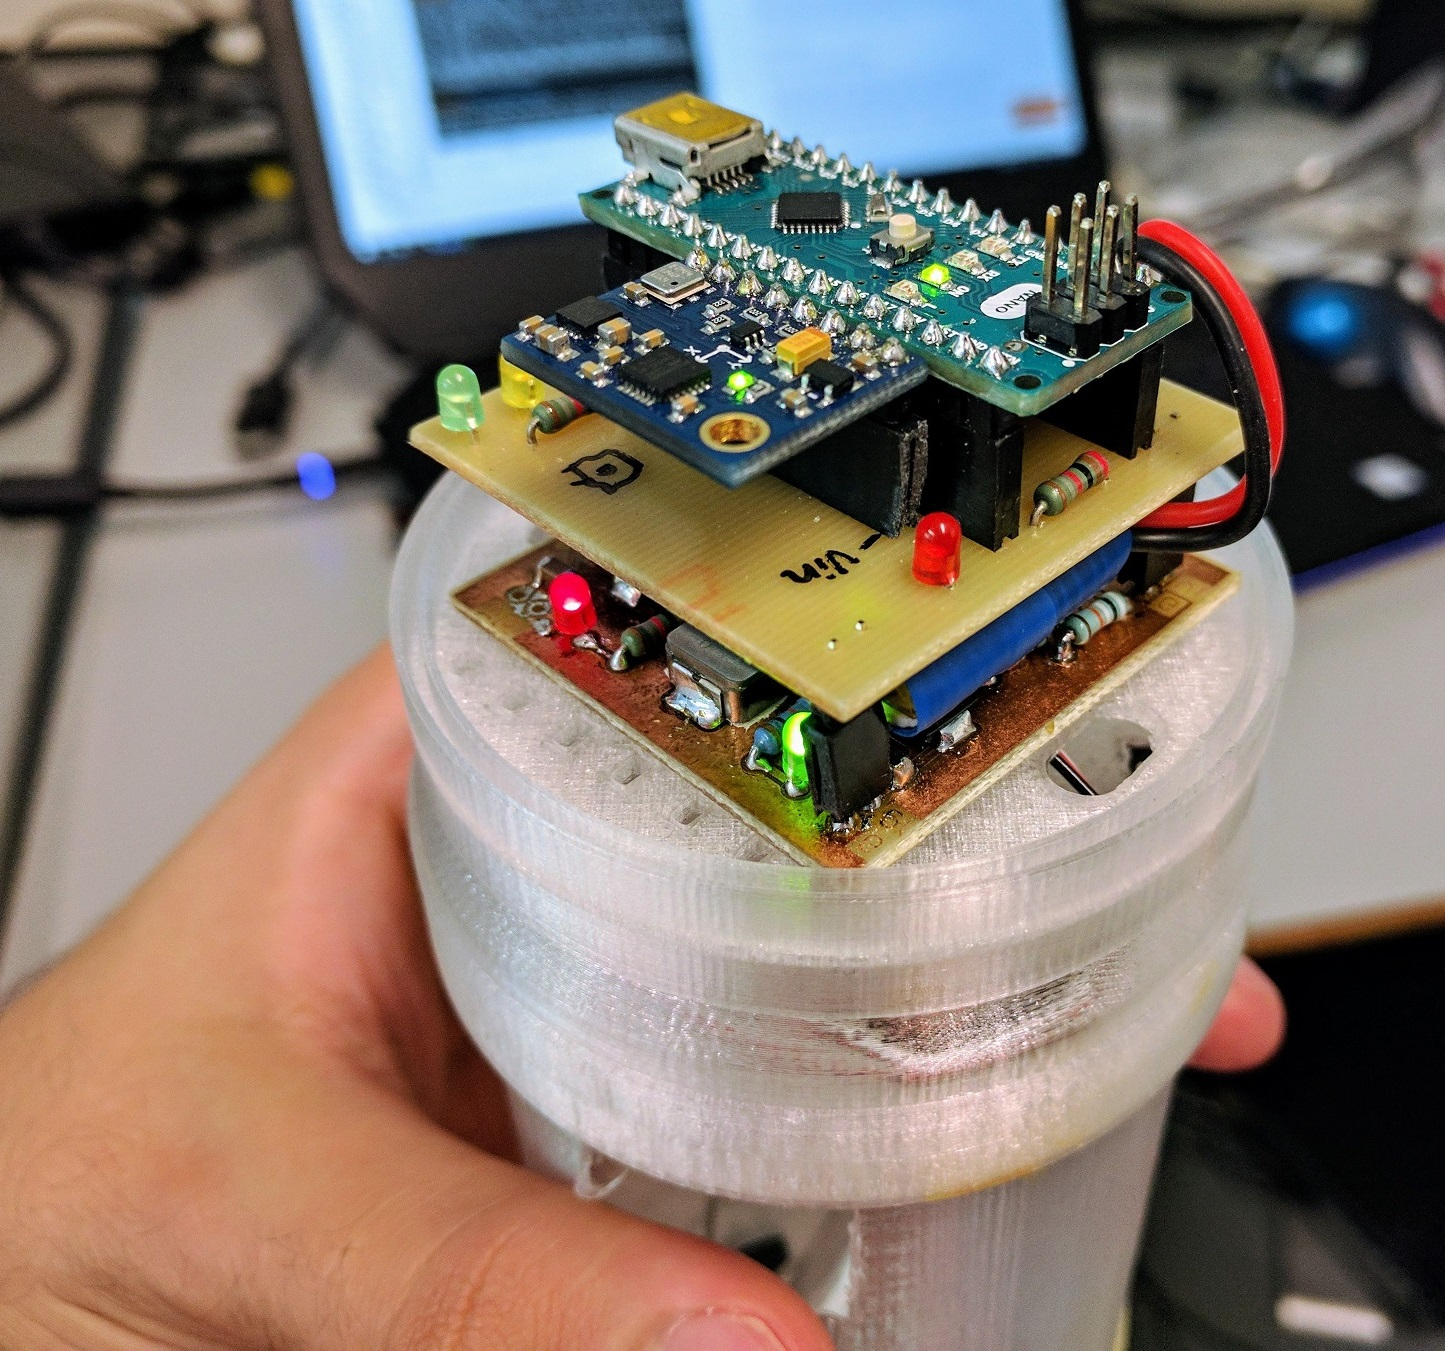
\includegraphics[width=0.8\linewidth]{figures/Rocket/implementation/assembled_PCBs.jpg}
	\caption{PCB stack assembled. Logic board on the top.}
	\label{fig:PCB_stack}
\end{figure}

The battery voltage is directed towards an analog input on the Arduino to be able to check the charge state, and possibly light a LED when the battery is below a threshold voltage. \\
This will be further discussed in the next session. The 3 other indicators are provided for debugging purposes.
The battery input is then passed by a connector to the PSU below, that provides the 5V rail to power the Arduino and the IMU.
$I^2C$ or Inter-Integrated Circuit, the protocol used to link the Arduino and the IMU needs two connections to operate.
\begin{itemize}
	\item SDA (Serial Data Line) : a bidirectional data line
	\item SCL (Serial Clock Line) : bidirectional clock synchronization line
\end{itemize}
They are connected to the dedicated $I^2C$ pins on the Arduino. \\
Last thing are the servo PWM (Pulse Width Modulation) output. \\
The Arduino produces a PWM signal to control the servo angle. The servomotor standard integrated controller interprets the angle command based on the duty cycle. 0\% is - 180$^{\circ}$ and 100\% is + 180$^{\circ}$. These PWM signals needs to be passed to the PSU board where the servo connector are (see next section).


\subsection{Power supply}
The rocket is electrically powered by a single cell 3.7V, 680 mAh LiPo battery. These batteries are lightweight, cheap, rechargeable and available in small form factors that fitted perfectly the rocket's size. \\

\begin{figure} [h]
	\centering
	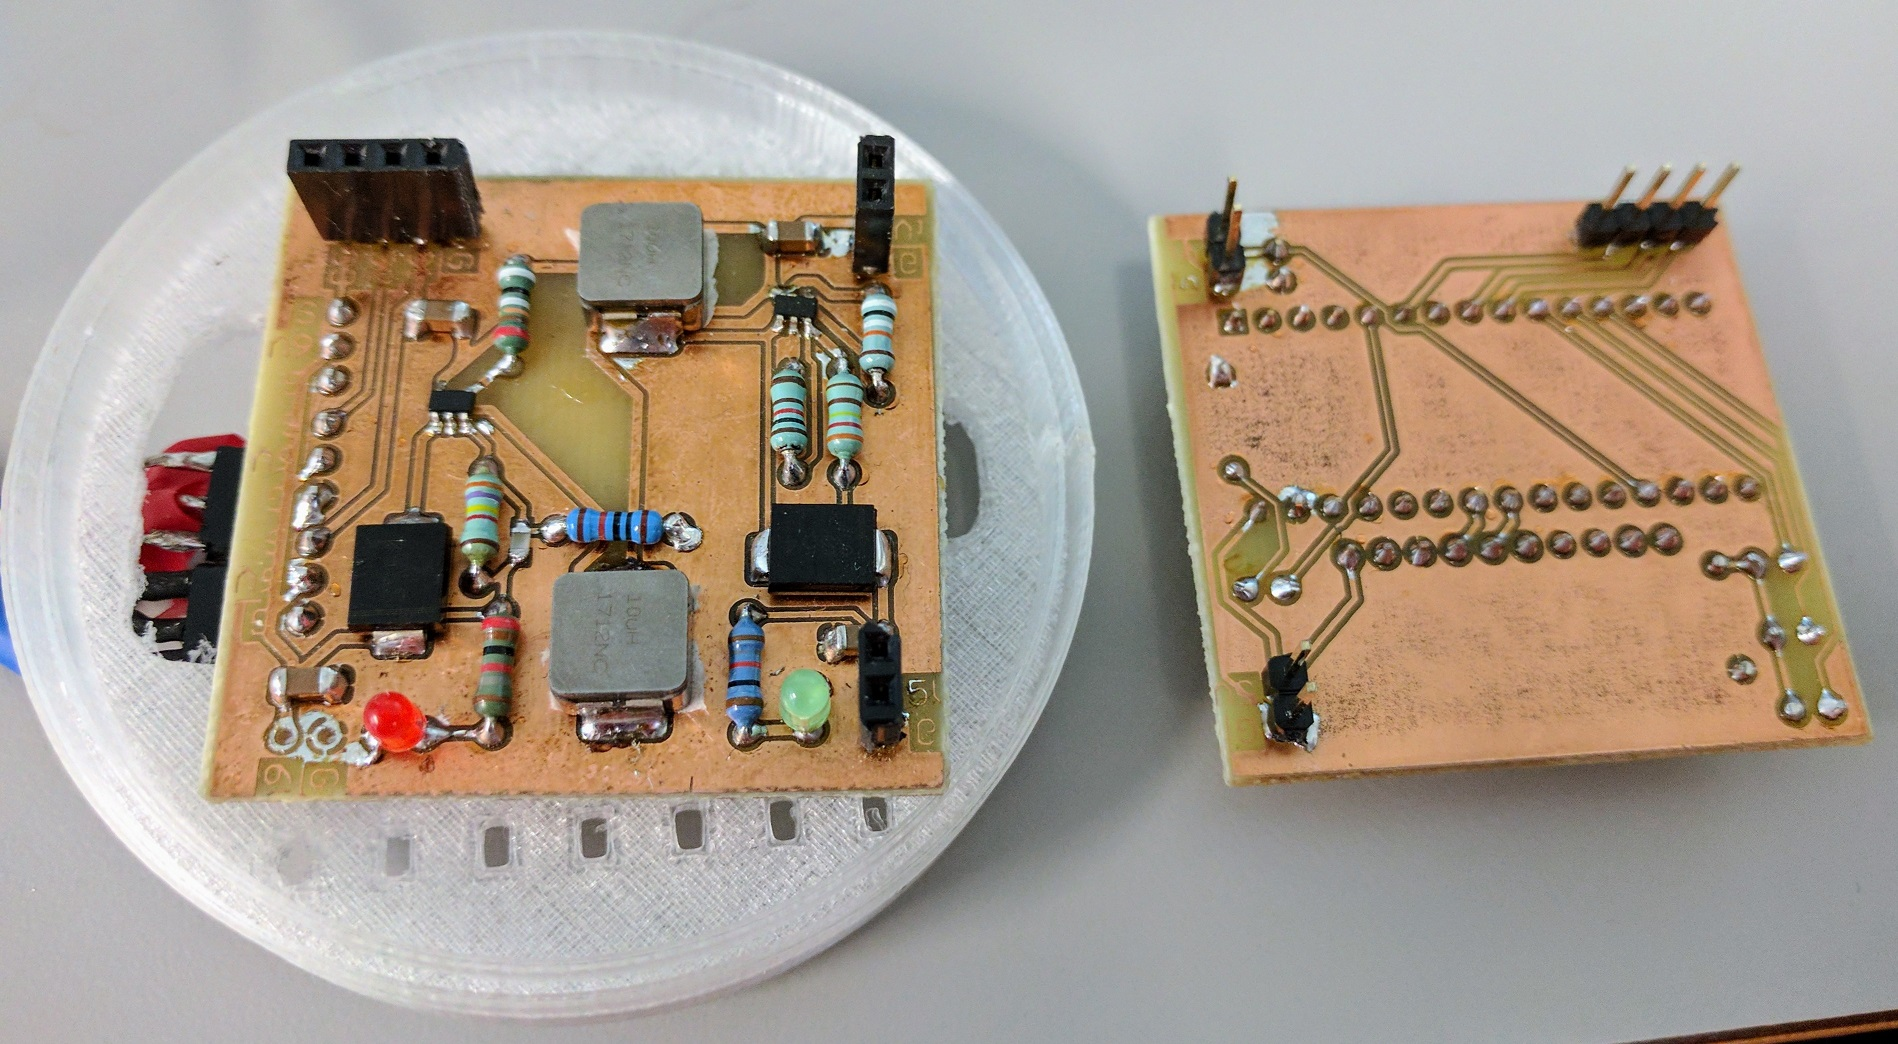
\includegraphics[width=0.8\linewidth]{figures/Rocket/implementation/psu_board.jpg}
	\caption{PCB stack disassembled. PSU on the left.}
	\label{fig:PSU_board}
\end{figure}

The logic components and the actuators must be very well separated since if they are not, a current draw spike on the actuator side could take all the available power and shutdown the logic components for a brief amount of time, causing them to reset, and the rocket to go out of control. \\
Since the logic and actuator parts of the power supply needed to be separated, two different power supplies were created on the same board (with common ground). \\
The logic side needs a 5V rail to function. The components are all powered by their Vin pin, which meant that they had a voltage stabilizer included. So the 5V output was set to 5.2V to compensate for the losses in the stabilizing circuit. \\
The actuators, namely the pitch and roll servos, were nano servos. As most standard servo can operate from 4.8V to 6V, they will be faster and have more torque at higher voltage. So the second power supply output was set to 6V. The servo test in \autoref{ssc:Servomotors} was done in these conditions. The servo connectors have 3 pins, PWM input was connected to the PWM output from the arduino, Vin was the 6V from the PSU, and the last pin is ground. \\
The PSU 5V rail was found to work at an input voltage as low as 3.6V input, but was supposed to work down to 2.5V. This was probably due to the lack of a feedback capacitor, even if the MIC2288YD5 datasheet's design advices \cite{datasheet:MIC2288} were not mentioning it. Anyways this minimum voltage was good enough for our use. The LED low battery indicator threshold was set to 3.65V.

\subsection{Igniter}
The igniter plugs that were available needed a 6V to 9V supply. 3-cell LiPo batteries are very common in the university, so the power was taken from a LiPo balancing plug, thus only using 2 cells to get 7.4V nominal voltage. The board is a very simple switch mechanism, the ignition needs to be armed first by flipping a switch before pushing the "fire" button. The PCB also features a protection capacitor, a buzzer and LEDs for user feedback.

\begin{figure} [h]
	\centering
	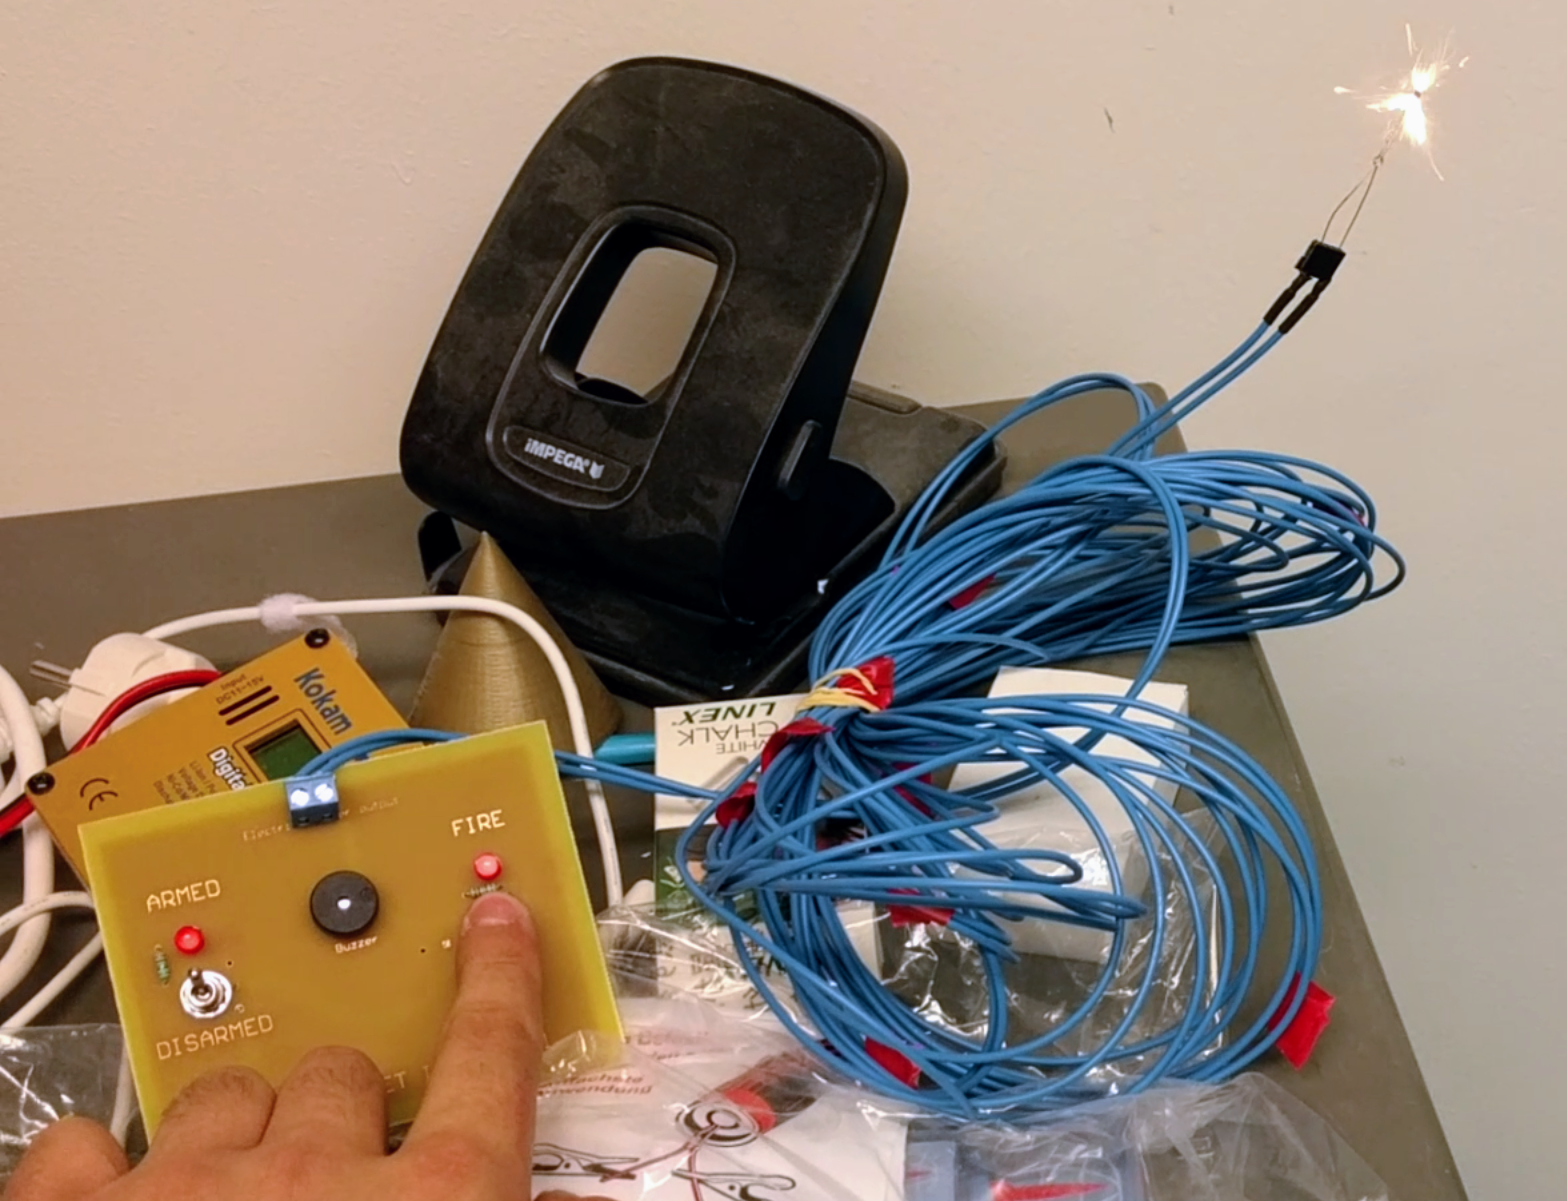
\includegraphics[width=0.8\linewidth]{figures/Rocket/implementation/igniter_PCB.png}
	\caption{PCB lighting an igniter with the PCB.}
	\label{fig:igniter_board}
\end{figure}

\section{Flight test}
The rocket was tested without the truster to check if the system was behaving correctly. A video of this test is included. The controller inclined the thruster in the correct direction according to the rocket's tilt.
A flight test was planned but delays in the rocket's construction did not allow to make the test safely and write the test report in time.
Strings would have been attached radially to the center of gravity of the rocket and to 2 sticks 3 meters apart. the wires would have been made long enough so the rocket would have been hovering slightly over the ground when idle, and the truster fired. This setup was inspired by a video found on Joe Lang's YouTube channel \cite{web:test_rocket}.
By filming the flight or logging the angle data on the Arduino's memory we could have seen the angle of inclination of the rocket during the attempt.